\part{Praxisteil}

\section{Versuchsaufbau}
Der Optimierungsversuch kann leider nicht auf dem Livesystem durchgeführt werden, da dass die Stabilität beeinträchtigen würde. Deswegen wurde ein Entwicklungssystem genutzt, um die verschiedenen Methoden zu analysieren. Dass Entwicklungssystem ist eine neuere Anschaffung der pludoni GmbH und dadurch im Vergleich zum Livesystem leistungsfähiger. Dadurch wird sich das Endergebnis, wenn es nach dem Abschluss der Arbeit auf das Livesystem übertragen wurde in seinen Kenndaten unterscheiden. Trotz alledem werden die Verbesserungen relativ zum Testsystem proportional ausfallen. 

\begin{itemize}
 \item Testplattform: pludoni Server eq4
  \item Prozessor: Intel® Core™ i7-920
  \item Arbeitsspeicher: 8 GB DDR3 RAM
  \item Festplatten: 2 x 750 GB SATA-II HDD (Software-RAID 1)
  \item Netzwerkverbindung: 100Mbit
  \item Server Software: Apache/2.2.16
  \item Server Hostname: itsax.it-jobs-und-stellen.de
  \item Server Port: 80
\end{itemize}

\section{Testverfahren}
Die rein serverseitigen Optimierungen wurden mit ab getestet. ab, das für apache bench steht, wurde entwickelt um Apache Server zu testen. Es analysiert wie lange ein Server braucht um Webseiten auszuliefern und wieviele Anfragen er pro Sekunde befriedigen kann, ohne das es zu Ausfällen kommt. Alle Änderungen die erst im Frontend, also im Browser, sichtbar werden wurden mit der Analyse von  webpagetest.org untersucht. Dabei wurden folgende Testparameter genutzt:
\begin{itemize}
  \item 10 konsekutive Tests (maximum) 
  \item Standort des Clients: Frankfurt a. M.
  \item Browser: IE9
  \item Connection: DSL 1,5 Mbps / 50ms RTT
  \item Only First View
\end{itemize}
Browsertests sind eine sehr komplizierte Angelegenheit, da es zum einen sehr viele Verschiedene Browser gibt und zum Anderen diese Browser in den verschiedensten Umgebungen ausgeführt werden. Ein Netbook zum Beispiel wird eine Webseite immer langsamer Darstellen, als ein Hexacore der neuesten Generation. Aus diesem Grund ist es von Vorteil eine Standardisierte Umgebung zu nutzen. Besonders die verschiedenen Analysen die automatisch durchgeführt werden sind positiv hervorzuheben:
\begin{itemize}
 \item Bewertung der Website nach den Google Page Speed Kriterien
 \item Inhaltsanalyse nach MIME Typen
 \item Performance Review in dem jedes Element der Homepage für sich betrachtet wird 
 \item Wasserfalldiagramm in dem schnell Problemzonen erkannt werden können
 \item Videovergleich des Seitenaufbaus mit anderen Webseiten
\end{itemize}
Andere Analyse Verfahren wie Profiling und Debugging auf Codeebene wurden nur sporadisch eingesetzt, da sie den Anwendungsfall Webseite nur eingeschränkt betreffen. Durch Caching kann der Server zum großen Teil vollständig entlastet werden und die Codeausführungszeit kann eliminiert werden.

\section{Ausgangszustand}
Sreeram Ramachandran ein Software Ingenieur der Firma Google hat eine Analyse über 4.2 Milliarden Seiten veröffentlicht. Diese ist im Rahmen der Initiative ``Let's make the web faster'' entstanden und zeigt häufige Fehlerquellen und ungenutztes Potential auf. Die durchschnittliche Webseite hat laut Ramachandran 320 kB Größe, 44 verschiedene Ressourcen und es werden nur 66\% der komprimierbaren Inhalte tatsächlich komprimiert.
Itsax.de hat 106 Ressourcen und 444 kB an Daten. Schon anhand dieser zwei Zahlen lässt sich eine vergleichsweise schwache Leistung vorhersehen. Besonders die Anzahl an verschiedenen Ressourcen deutet auf Missstände hin, da Parallelisierung von Zugriffen nur bis zu einem bestimmten Grad möglich ist. Die Time to First Byte(TtFB) von 674ms bezeichnet die Zeit die vergeht bis der Webbrowser die ersten Daten empfängt, dass bedeutet aber noch nicht das der Nutzer schon Inhalte präsentiert bekommt. Die Inhalte werden erst angezeigt nachdem die Time to Start Render(TtSR) vergangen ist, der Nutzer muss demnach ungefähr zwei Sekunden warten bis die Webseite im Browser anfängt sich aufzubauen. Die Load Time(LT) bezeichnet dann die Zeit die vergeht bis die Seite komplett dargestellt wird und der Benutzer sie ohne Einschränkungen bedienen kann. Es können  aber auch nach der LT noch Inhalte nachgeladen werden, wie zum Beispiel gestreamte Videos oder andere asynchrone Inhalte. Diese nachgeladenen Inhalte wirken sich aber nicht mehr Negativ auf die User Experience aus, solange sie im Rahmen bleiben und nicht wichtige Teile der Webseite wie zum Beispiel das Hauptmenü noch per Flash geladen werden müssen. Die Anzahl der DOM Elemente bezeichnet alle vom Browser zu verarbeitenden Objekte und ist ein Indikator für die Komplexität der Webseite, je mehr Elemente also vorhanden sind desto länger muss der Browser die Positionierung und Darstellung berechnen. Die Inhalte auf der Seite Itsax.de sind in Abbildung ? dargestellt, einmal im Bezug auf Größe und einmal aufgeschlüsselt nach der Anzahl der benötigten Requests um die Inhalte vom Server anzufordern. Die folgenden Ergebnisse wurde mit dem Analysetool webpagetest.org ermittelt. Leicht zu erkennen ist, dass der HTML Anteil sowohl bei der Größe als auch bei Anzahl der HTTP Anfragen eine Untergeordnete Rolle spielt. Nicht vergessen werden darf aber die Zeit die der Server benötigt um den HTTP Code zu generieren. Dies kann man sehr gut in einem Wasserfalldiagramm erkennen, in dem der Start des Ladevorgangs hervorgehoben wurde. Bevor der initiale GET Request abgeschlossen ist, weiss der Browser noch nicht welche Ressourcen er laden muss und es können noch keine anderen Aktionen ausgeführt werden.
\begin{figure}[htbp]
  \centering
  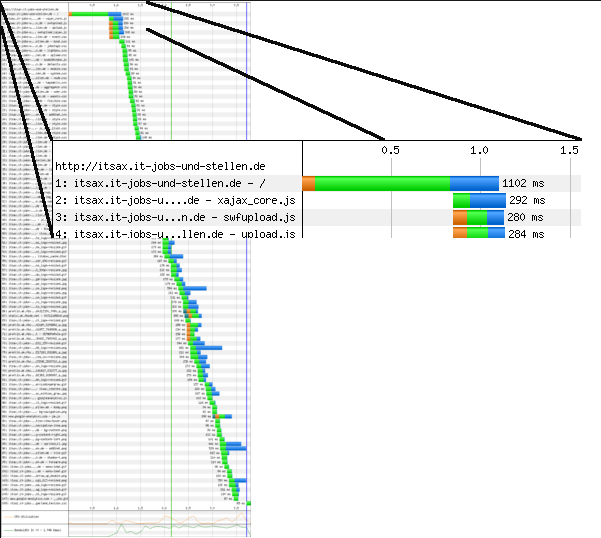
\includegraphics[scale=0.5]{material/start_waterfall_edited.png}
  \caption{Wasserfalldiagramm: Ausgangszustand}
  \label{fig:startwaterfall}
\end{figure}
\begin{figure}[htbp]
  \centering
  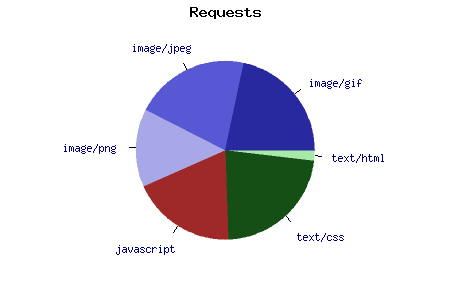
\includegraphics[scale=0.5]{material/start_request_pie.png}
  \caption{HTTP Anfragen}
  \label{fig:startrequest}
\end{figure}

\begin{figure}[htbp]
  \centering
  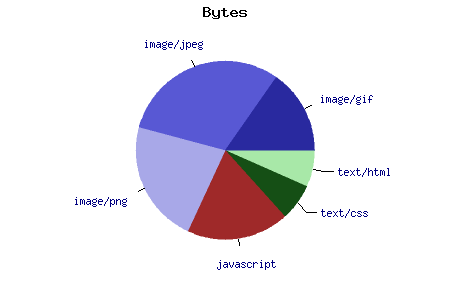
\includegraphics[scale=0.5]{material/start_byte_pie.png}
  \caption{Größe der Inhalte}
  \label{fig:startbyte}
\end{figure}

Load Time: 3.728
Time to First Byte: 0.674s 	
Time to Start Render: 2.002s
\#DOM Elements: 855 	
\#Requests: 106
Bytes In: 444 kB
\begin{tabbing}
Request \quad\= blablabla \quad\= \kill
\textbf{Typ} 	 \> \textbf{Anzahl} \\
text/css	 \>	24 	\\
image/gif	 \>	23 	\\
image/jpeg	 \>	22 	\\
javascript	 \>	20 	\\ 
image/png	 \>	15 	\\
text/html	 \>	2 	\\
\end{tabbing}

\begin{tabbing}
Request \quad\= blablabla \quad\= \kill
\textbf{Typ} 	 \> \textbf{Byte} \\
image/jpeg	\>142251\\
image/png	\>101428\\
javascript	\>84758\\
image/gif	\>73378\\
text/css	\>30222\\
text/html	\>29917\\

\end{tabbing}
%http://code.google.com/intl/de/speed/articles/web-metrics.html


Document Path:          /
Document Length:        65218 bytes

Concurrency Level:      1
Time taken for tests:   18.182 seconds
Complete requests:      50

Write errors:           0
Total transferred:      3266726 bytes
HTML transferred:       3239226 bytes
Requests per second:    2.75 [\#/sec] (mean)
Time per request:       363.640 [ms] (mean)
Time per request:       363.640 [ms] (mean, across all concurrent requests)
Transfer rate:          175.46 [kBytes/sec] received



\section{Implementierung und Test der einzelnen Methoden}
Im folgenden Abschnitt werden die eingesetzten Methoden dargestellt und ihre Auswirkungen auf die Webperformance der Seite itsax.de dargestellt. 
In diesem Abschnitt werden alle Methoden die vom Autor, nach der Analyse des Ausgangszustands, für möglicherweise sinvoll befunden wurden getestet. Die Methode wird jeweils mit dem Startwert verglichen und der Aufwand wird eingeschätzt.
\subsection{APC}
Server Software:        Apache/2.2.16
Server Hostname:        itsax.it-jobs-und-stellen.de
Server Port:            80

Document Path:          /
Document Length:        64842 bytes

Concurrency Level:      1
Time taken for tests:   11.681 seconds
Complete requests:      50

Write errors:           0
Total transferred:      3261730 bytes
HTML transferred:       3234230 bytes
Requests per second:    4.28 [\#/sec] (mean)
Time per request:       233.620 [ms] (mean)
Time per request:       233.620 [ms] (mean, across all concurrent requests)
Transfer rate:          272.69 [kBytes/sec] received

\subsection{Drupal Cache}
Server Software:        Apache/2.2.16
Server Hostname:        itsax.it-jobs-und-stellen.de
Server Port:            80

Document Path:          /
Document Length:        65005 bytes

Concurrency Level:      1
Time taken for tests:   2.082 seconds
Complete requests:      50
Failed requests:        0
Write errors:           0
Total transferred:      3276900 bytes
HTML transferred:       3250250 bytes
Requests per second:    24.02 [\#/sec] (mean)
Time per request:       41.638 [ms] (mean)
Time per request:       41.638 [ms] (mean, across all concurrent requests)
Transfer rate:          1537.09 [kBytes/sec] received


%http://www.webpagetest.org/result/110809_BH_198S4/


\subsection{JS Aggregation und Minifizierung mit dem Javascript Aggregation Modul}
Aggregation und Minifizierung sind Verfahren, die in der Webperformance Optimierung häufig eingesetzt werden. Für das Drupal 5 System gibt es fertige Module die diese Aufgabe übernehmen. Das Modul interveniert innerhalb des Drupal Kerns und ersetzt die Javascripts, die vorher direkt so ausgegeben wurden wie sie die Module lieferten, durch eine einzelne, das heisst aggregierte Version, die optional minifiziert werden kann. Diese Minifizierung wird natürlich genutzt und spart einige kB. Minifizierung wird ermöglicht durch die Nutzung von JSmin https://github.com/rgrove/jsmin-php/. JSmin ist ein Filter der unter anderem Kommentare entfernt und mehrere Leerzeichen zu einem zusammenfasst. Durch die Nutzung dieser Methode konnten 11 HTTP Abfragen und 11 kB an Datenvolumen eingespart werden.
Load Time: 3.658s
Time to First Byte: 0.595s
Time to Start Render: 1.915s
\#DOM Elements: 844 	
\#Requests: 95 %!
Bytes In: 432 kB
%http://www.webpagetest.org/result/110809_Z1_198TK/

\subsection{CSS Aggregation und Komprimierung}
Analog zur Javascript Optimierung kann man auch die CSS Aggregation betrachten. Dabei werden durch Zusammenfassung der einzelnen CSS Dateien HTTP Abfragen eingespart. Wie man an der gesunkenen Anzahl der Requests sehen kann, wurden 21 Abfragen nur durch Zusammenfügen der einzelnen CSS Dateien zu einer einzigen eingespart. Durch die Bereinigung beziehungsweise Komprimierung werden dabei außerdem 17 kB an überflüssigen Zeichen entfernt. 
Load Time: 3.577s
Time to First Byte: 0.649s
Time to Start Render: 1.577s
\#DOM Elements: 834 	
\#Requests: 85 %!
Bytes In: 427 kB
%http://www.webpagetest.org/result/110809_XB_198VE/
\subsection{Drupal Boost Module}
Load Time: 3.233s
Time to First Byte: 0.172s %!
Time to Start Render: 1.473s
\#DOM Elements: 856 	
\#Requests: 106 %!
Bytes In: 444 kB
%http://www.webpagetest.org/result/110809_AP_198XJ/

\subsection{Bildoptimierungen mit jpegoptim und OptiPNG verlustfrei!}
Bilder und Grafiken bieten oft großen Optimierungsspielraum. Zum einen erfolgt dies durch die richtige Auswahl der Dateiformate und zum anderen durch Komprimierung der Bilder. Da es auf www.itsax.de nicht nur statische Inhalte gibt, sondern auch durch Communitymitglieder und Communitymanager eingestellte Inhalte verwaltet werden müssen, sollte eine nachträgliche Qualitätsoptimierung der hochgeladenen Bilder durchgeführt werden. Um dies umzusetzen, sind die Programme OptiPNG und jpegOptim zu empfehlen. Auf jeden Fall sollte eine verlustfreie Komprimierung durchgeführt werden, da die Bilder in diesem Fall nur an Dateigröße verlieren und die Bildqualität unberührt bleibt. Da es sich bei beiden Programmen um Kommandozeilenprogramme handelt, kann man ihre Anwendung leicht automatisieren. Mit dem Linuxbefehl find, der praktischerweise eine Möglichkeit, Befehle auszuführen, besitzt, kann man direkt die entsprechenden Dateien an die Optimierer übergeben. Diese Aktionen können dann über einen Cronjob periodisch jede Nacht ausgeführt werden. Die Befehle sehen dann wie folgt aus: 
find . -name "*.png" -exec optipng -o7 {} \;
find . -name "*.jpg" -exec jpegoptim {} \;

%%http://optipng.sourceforge.net/
%%http://www.kokkonen.net/tjko/projects.html

Load Time: 3.640
Time to First Byte: 0.636s %!
Time to Start Render: 1.894s
\#DOM Elements: 855 	
\#Requests: 106 %!
Bytes In: 429 kB % 15kb gespart
%http://www.webpagetest.org/result/110809_C4_1999C/
\subsection{Bildoptimierungen mit OptiPNG verlustfrei und mit jpegoptim verlustbehaftet! 50\% kompression}
find . -name "*.png" -exec optipng -o7 {} \;
find . -name "*.jpg" -exec jpegoptim {} \;

Load Time: 3.255s
Time to First Byte: 0.669s %!
Time to Start Render: 1.908s
\#DOM Elements: 855 	
\#Requests: 106 %!
Bytes In: 371 kB % 73kb gespart
%http://www.webpagetest.org/result/110809_15_199GY/

\subsection{Drupal 5 Fehler bei umgefärbten Themes}
Das Framework Drupal 5 benutzt Themes zur Gestaltung der Oberfläche. Um diese farblich anpassen zu können, wurde das Color Modul installiert, welches Themeveränderungen ermöglicht. Aufgrund der Tatsache, dass das Theme nur kopiert wird und im Anschluss die Farben geändert werden, entstehen bei diesem Vorgang unnötige Duplikate, die beim Laden der Seite mitgeschleppt werden. Um diese zu entfernen, wird einfach das Standardtheme durch das Modifizierte ersetzt. Dafür müssen  nur noch einige Pfade in der style.css angepasst werden und man spart in dem Fall von itsax.de 4 kB, was immerhin ca 1\% der übertragenen Datenmenge ausmacht.
händisch gemergte styles
style auf standard setzen
vorher die images und das geänderte stylesheet kopieren
Load Time: 3.626s
Time to First Byte: 0.629s %!
Time to Start Render: 1.890s
\#DOM Elements: 854 	
\#Requests: 104 %!
Bytes In: 440 kB % 4kb gespart
%http://www.webpagetest.org/result/110809_SZ_19APH/

\subsection{Theme Bilder Spriten}
Spriting wurde ursprünglich in der Videospielentwicklung verwendet, um Bilder in den Grafikspeicher zu laden. In der Webentwicklung ist es eine effektive Technik, um Bilder ohne mehrfachen Overhead zu laden. Beim Spriting wird aus vielen einzelnen Bildern ein einziges Bild erstellt, dass anstelle der vielen Bilder geladen wird. Um die Bilder dann noch einzeln Anzeigen zu können, werden CSS Befehle genutzt, die es ermöglichen, die Größe und die Position eines Bildausschnittes anzuzeigen. 
Load Time: 3.707
Time to First Byte: 0.669s %!
Time to Start Render: 1.968s
\#DOM Elements: 855 	
\#Requests: 103 
Bytes In: 443 kB 
%http://www.webpagetest.org/result/110810_FZ_19GBA/

\subsection{Verschiedene Module von Startseite entfernen}
Um zu überprüfen, welchen Einfluss verschiedene, im Netzwerkgraphen auffällige, Module auf die Gesamtperformance haben, werden sie testweise komplett deaktiviert. So kann man entscheiden, bei welchen Modulen zusätzlicher Programmieraufwand lohnenswert ist.
Partnerslideshow:
Load Time: 2.695s
Time to First Byte: 0.636s %!
Time to Start Render: 1.838s
\#DOM Elements: 790
\#Requests: 80
Bytes In: 276 kB
%http://www.webpagetest.org/result/110810_JT_19HS5/

facebook fenster:
Load Time: 3.478s
Time to First Byte: 0.668s %!
Time to Start Render: 1.966s
\#DOM Elements: 779 	
\#Requests: 95 
Bytes In: 406 kB 
%http://www.webpagetest.org/result/110810_63_19HZT/

Jobleiste deaktiviert:
Load Time: 3.367s
Time to First Byte: 0.617s %!
Time to Start Render: 1.709s
\#DOM Elements: 822 	
\#Requests: 94 
Bytes In: 411 kB
%http://www.webpagetest.org/result/110810_4F_19J8H/

\subsection{Umprogrammierung verschiedener Module}
Um die langsamen Module weiterhin nutzen zu können, muss eine Lösung gefunden werden, die es ermöglicht, Inhalte nachzuladen, nachdem die Seite komplett geladen wurde. Um das zu erreichen, kann man mit der Hilfe von Javascript bestimmte DOM Elemente über einen Timeoutbefehl erst nachdem der Browser gemeldet hat er hat die Seite fertig geladen, die Inhalte nachladen.
Partnerslideshow:
Load Time: 2.749s (3.794)
Time to First Byte: 0.626s %!
Time to Start Render: 1.842s
\#DOM Elements: 855 	
\#Requests: 82 (107)
Bytes In: 284 kB (395)
%http://www.webpagetest.org/result/110810_3Z_19MRE/

facebook fenster:
Load Time: 3.411s (4.258)
Time to First Byte: 0.576s %!
Time to Start Render: 1.848s
\#DOM Elements: 857
\#Requests: 95 (106)
Bytes In: 406 kB (444)
%http://www.webpagetest.org/result/110810_AJ_19N72/

Partneranzeigen:
Load Time: 3.871s (5.759s)
Time to First Byte: 0.669s %!
Time to Start Render: 2.255s
\#DOM Elements: 857 	
\#Requests: 105 (108)
Bytes In: 417 kB (448)
%http://www.webpagetest.org/result/110815_N6_1AWKT/1/details/


\section{Endergebnis}
Die Ladezeiten haben sich gravierend Verbessert, weniger als die Hälfte der Zeit wird benötigt bis die Seite benutzbar ist.

Load Time: 1.354s (2.913s)
Time to First Byte: 0.173s %!
Time to Start Render: 0.952s
\#DOM Elements: 789 	
\#Requests: 25 (67)
Bytes In:  138 kB (314)
%http://www.webpagetest.org/result/110825_5J_1DQHK/
